\section{Modelo proposto}

O modelo proposto foi inspirado pelos conceitos de ilusão e alucinação apresentados na Seção \ref{anomalias}, que o nomeiam -- o nome HAIL vem da junção das palavras \textit{hallucination} e \textit{illusion}, alucinação e ilusão em inglês, respectivamente. Seu objetivo é identificar anomalias nas percepções recebidas por um agente qualquer e torná-las informação úteis na forma de novos planos.

O modelo HAIL foi desenvolvido para que seja possível adicioná-lo a qualquer agente, independente de arquitetura cognitiva, como um componente que conecta as percepções vindas do ambiente ao agente. O HAIL pode ser separado em dois módulos, como mostra a Figura \ref{fig:method}. De maneira geral, o funcionamento e a comunicação desses módulos se dá da seguinte maneira:

\begin{enumerate}
    \item As percepções recebidas pelo modelo são refinadas pelo módulo de refinamento;
    \item As percepções refinadas passam pelo módulo de alucinação e ilusão onde são categorizadas entre:  percepções válidas, alucinações, ilusões classe 1 e ilusões classe 2. 
    \item As percepções válidas são encaminhadas para o raciocínio do agente, enquanto as anomalias continuam no módulo de alucinação e ilusão armazenadas em estruturas chamadas de bloco avaliador;
    \item Quando os requisitos estabelecidos pelo bloco avaliador são cumpridos, as anomalias são selecionadas para passarem pelo processo de planejamento automatizado, alimentando o agente com novos planos.
\end{enumerate}
    
\begin{figure}[h!]
    \centering
    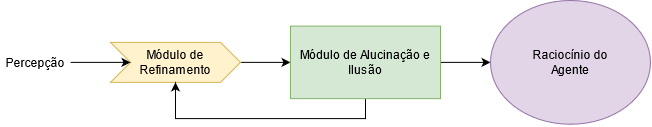
\includegraphics[width=1\textwidth]{images/modelo_geral.png}
    \caption{Visão geral do modelo HAIL.}
    \label{fig:method}
\end{figure}

\subsection{Módulo de refinamento}

\label{refinamento}

O módulo de refinamento funciona como uma primeiro filtro para que percepções indesejadas pelo agente não cheguem até seu ciclo de raciocínio. O processo de refinamento é descrito pela Definição \ref{def:refinamento}.

O processo de refinamento não é obrigatório. Caso não seja de interesse de uma determina implementação do HAIL refinar suas percepções, basta que a função do módulo de refinamento seja a função identidade $f(x) = x$, possuindo assim $\rho = p$.

\subsection{Módulo de alucinação e ilusão}

\begin{figure}[h]
    \centering
    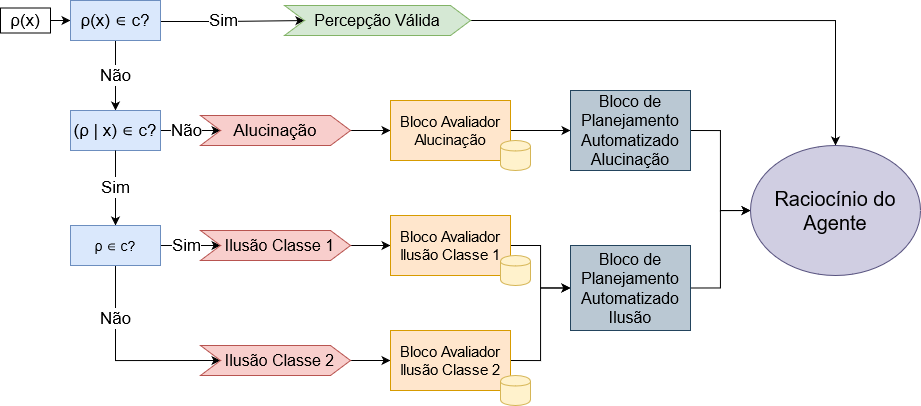
\includegraphics[width=1\textwidth]{images/diagrama-modelo.png}
    \caption{Módulo de alucinação e ilusão.}
    \label{fig:model}
\end{figure}
 
 A Figura \ref{fig:model} apresenta um diagrama do funcionamento do módulo de alucinação e ilusão. Sua função é receber todas as percepções que passaram pelo processo de refinamento, e detectar quais delas são anomalias. Para isso, esse módulo utiliza uma cadeia de decisores descrita pelo Algoritmo \ref{algorithm:decisor}. Depois de serem classificadas pelos decisores, as anomalias são guardadas em seus respectivos blocos avaliadores.

\begin{algorithm}[H]
\Entrada{contexto \textit{c} do agente, percepção $\rho(x)$}
\Inicio{
 \label{algorithm:decisor}
  \uSe{$\rho(x)$ está em \textit{c}}{
  $\rho(x)$ é uma percepção válida\;
  }\uSenaoSe{nem $\rho$ nem $x$ estão em c}{
  $\rho(x)$ é uma alucinação\;
  }\uSenaoSe{$\rho$ está em \texttt{c}}{
  $\rho(x)$ é uma ilusão classe 1\;
  }\Senao{$\rho(x)$ é uma ilusão classe 2}
}
 \caption{Funcionamento dos decisores do módulo de alucinação e ilusão.}
\end{algorithm}

\subsubsection{Bloco avaliador}

O objetivo do bloco avaliador é decidir quando alucinações e ilusões que foram recebidas devem ser processadas, evitando que o planejamento automatizado que será realizado em seguida tenha impacto no tempo de execução de um ciclo de raciocínio do agente. Para isso, utilizamos uma lista ordenada por peso como escalonador. O principio do funcionamento da lista ordenada por peso é o mesmo de uma fila, \textit{first in first out} (FIFO), mas atribui um peso a cada entrada que aumenta quando novos elementos iguais são inseridos. Quando um elemento é inserido pela primeira vez na fila, ele recebe o peso 1, e quando uma cópia do mesmo elemento é inserida o elemento tem seu peso aumentado em 1. Quando uma operação de remoção é executada, o elemento de maior peso é removido. Se dois ou mais elementos tiverem o maior peso, aquele que foi inserido primeiro é removido.

O bloco avaliador seleciona quando uma percepção deve ser tratada através de uma função matemática, levando em conta o tempo médio de processamento de uma percepção válida e de uma anomalia. Além desse funcionamento básico, o bloco avaliador ainda contém um mecanismo para remover anomalias classificadas com irrelevantes para o sistema, através de uma função de limpeza. Caso essa função retorne verdadeiro, todos os elementos de peso 1 da sua respectiva lista são removidos. Essas duas funções são descritas com mais detalhes na Seção \ref{section:formalizacao}.

\subsubsection{Bloco de planejamento automatizado}

O bloco de planejamento automatizado é potencialmente a parte mais custosa computacionalmente, o que pode ser um gargalo do sistema, principalmente caso o agente funcione em tempo real e receba um volume muito elevado de percepções por segundo. Um planejamento automatizado implementado de maneira puramente simbólica tende a ser complexo computacionalmente, uma vez que pode considerar milhares de alternativas para o estado de mundo atual, tentando chegar mais perto de seu objetivo. Um processo de planejamento automatizado conexionista é uma alternativa, uma vez que estamos tratando de uma análise incompleta do mundo. Caso seja possível, teorias com maior custo computacional (como criatividade computacional \cite{colton2012computational}) podem ser aplicadas aqui para um resultado ainda mais preciso.

Uma percepção chega ao bloco de planejamento automatizado uma vez que ela seja a primeira na fila ponderada e a função de processamento retorne verdadeiro em sua verificação. De um ciclo para outro, as percepções permanecem na fila, a não ser que sejam descartadas pelo mecanismo de limpeza. Nosso modelo não explicita qual é a ordem que os blocos avaliadores devem processar suas filas para mandar anomalias para o planejamento automatizado (isto é, se deve primeiro ser priorizada as anomalias do bloco avaliador de alucinações, ilusões classe 1 ou ilusões classe 2), ficando a cargo da implementação em questão tomar essa decisão.

\subsection{Formalização}

\label{section:formalizacao}

O bloco básico do modelo de revisão de percepções proposto, chamado de HAIL, é composto por um módulo para alucinação e ilusão $M_{ai}$ e uma função de refinamento $\theta$, conforme descrito na Definição \ref{def:modeloHAIL}. O módulo de ilusão e alucinação é uma quádrupla, apresentada na definição \ref{def:illuHallu}. A função de refinamento é uma função abstrata, cuja entrada é obtida através dos sensores do agentes e a saída é a entrada do módulo de alucinação e ilusão, conforme já foi descrito anteriormente na Seção \ref{refinamento}.
 
 \vspace{0.2cm}
 
 \begin{definition}{}
    O modelo de revisão de percepções HAIL é uma dupla $HAIL = \langle M_{ai}, \theta \rangle$, onde:
    
    \begin{itemize}
        \item $M_{ai}$ é o módulo de ilusão e alucinação; e
        \item $\theta$ é a função de refinamento $\theta(p) = \rho$, onde $p$ é um conjunto de percepções e $\rho$ é um subconjunto próprio de $p$.
    \end{itemize}{}
    \label{def:modeloHAIL}
\end{definition}

Após ter passado pela função $\theta$, as percepções $\rho$ irão passar pelo Algoritmo \ref{algorithm:decisor}, e serão encaminhadas de acordo com sua classificação. O bloco de ilusão e alucinação é descrito por uma quádrupla, com conjuntos de decisores, blocos e uma função de transição.

\vspace{0.2cm}

\begin{definition}
\label{def:illuHallu}
    O bloco de ilusão e alucinação é uma quádrupla $M_{ai} = \langle D, Ab, Ap, \Delta \rangle$, onde:
    
    \begin{itemize}
        \item $D$ é o conjunto de decisores $D = \{d_{a}, d_{h}, d_{i}\}$, onde:
             \begin{itemize}
                \item $d_{a}$ é o decisor de anomalias, definido pela função:
                \[ d_{a} = \left\{ \begin{array}{ll}
                0 & \mbox{se $\rho(x)$ está em $c$\footnotemark};\\
                1 & \mbox{se $\rho(x)$ não está em $c$}.\end{array} \right. \]
             
                \item $d_{h}$ é o decisor de alucinação, definido pela função:
                \[ d_{h} = \left\{ \begin{array}{ll}
                0 & \mbox{se nem $\rho$ nem $(x)$ está em $c$};\\
                1 & \mbox{se $\rho$ ou $(x)$ está em $c$}.\end{array} \right. \]
                
                \item $d_{i}$ é o decisor de ilusão, definido pela função:
                \[ d_{i} = \left\{ \begin{array}{ll}
                0 & \mbox{se $\rho$ está em $c$};\\
                1 & \mbox{se $(x)$ está em $c$}.\end{array} \right. \]
            \end{itemize}
        
        \footnotetext{ $c$ é o contexto do agente, de acordo com a definição \ref{definition::context}.}
        
        \item $Ab$ é o conjunto de blocos avaliadores $Ab = \{Ab_{h}, Ab_{i1}, Ab_{i2}\}$, onde $Ab_{h}$ é o bloco avaliador de alucinações, $Ab_{i1}$ é o bloco avaliador de ilusões classe 1 e $Ab_{i2}$ é o bloco avaliador de ilusões classe 2.
        
        \item $Ap$ é o conjunto de blocos de planejamento automatizado $Ap = \{Ap_{h}, Ap_{i}\}$, onde $Ap_{h}$ é o bloco de planejamento automatizado de alucinações e $Ap_{i}$ é o bloco de planejamento automatizado de ilusões.
        
        \item $\Delta$ é a função de transição definido pela tabela abaixo, onde $out$ é um estado final, que leva a percepção para fora do modelo de revisão de percepções, ou seja, pode tanto significar o encaminhamento de uma percepção válida para o raciocínio do agente quanto o fim da execução de um ciclo de revisão.
        
            \begin{table}[htb]
                \caption{Função de transição $\Delta$ do módulo de ilusão e alucinação.}
                \centering
                \begin{tabular}{c c c c} 
                    \toprule
                    \textbf{Estado} & \textbf{0} & \textbf{1} \\
                    \midrule
                    $d_{a}$     & $out$     & $d_{h}$       \\
                    $d_{h}$     & $Ab_{h}$  & $d_{i}$       \\
                    $d_{i}$     & $Ab_{i1}$ & $Ab_{i2}$     \\
                    $Ab_{h}$    & $out$     & $Ap_{h}$      \\
                    $Ab_{i1}$   & $out$     & $Ap_{i}$      \\
                    $Ab_{i2}$   & $out$     & $Ap_{i}$      \\
                    \bottomrule
                \end{tabular}
                \label{transition-table}
                
            \end{table}
    \end{itemize}{}
\end{definition}{}

O módulo de ilusão e alucinação é o artefato principal do modelo. Ele é subdividido em três partes principais: os decisores, os blocos avaliadores e os blocos de planejamento automatizado. Seu comportamento é descrito por uma função de transição que define o estado atual do módulo.

\vspace{0.2cm}

\begin{definition}
    Um bloco avaliador é uma tripla $Ab_{x} = \langle L, Pf, Cf) \rangle$, $x \in \{h, i1, i2\}$, onde:

    \begin{itemize}
        \item $L$ é uma lista ordenada pelo número de vezes que uma mesma anomalia é dada como entrada;
        \item $Pf$ é a função de processamento, definida abaixo:
            
             \[ Pf = \left\{ \begin{array}{ll}
                        1 & \mbox{se $T_{m}(A) \leq T_{m}(V) * (|A| - |A_{pr}|)$;}\\
                        0 & \mbox{caso contrário}.\end{array} \right. \]
        
            
            Onde:
            
            \begin{itemize}
                \item $T_{m}$ é a função que retorna a média do tempo gasto para processar as percepções de um conjunto;
                \item $A$ é o conjunto de anomalias, $A(x)$ é um elemento específico $x$ e $|A|$ o número de anomalias do conjunto;
                \item $A_{pr}$ é o conjunto de anomalias que já foram validadas para serem processadas pela função de processamento neste ciclo de raciocínio ($A_{pr}$ é instanciada vazia a cada ciclo de raciocínio), e $|A_{pr}|$ o número de anomalias desse conjunto.
                \item $V$ é o conjunto de percepções válidas.
            \end{itemize}{}
        
        \item $Cf$ é a função de limpeza definida abaixo com auxílio da função equação de limpeza $Cf$, sendo $\alpha$ um coeficiente de limpeza variável que precisa ser definido pela instância implementada do modelo (por padrão, toma-se $\alpha = 1$):
        
        \[ Cf = \left\{ \begin{array}{ll}
                        1 & \mbox{se  $Ce = Verdadeiro$;}\\
                        0 & \mbox{caso contrário}.\end{array} \right. \]
            
            \[ Ce = \sum_{i=1}^{|L|} W_{n}(L_{i}) > \alpha \sum_{j=1}^{|L|} W_{1}(L_{j}) \]
            
            Onde:
            
            \begin{itemize}
                \item $L$ é a lista ordenada do bloco, sendo $|L|$ seu número de anomalias e $L_{i}$ a anomalia $i$ da lista.
                \item $W$ é a função peso da anomalia $L_{i}$ definida como $W(L_{i}) = |L_{i}|$, sendo $|L_{i}|$ o peso da anomalia especificada (número de entradas recebidas dessa mesma anomalia na lista). A função $W$ é utilizada para especificar as seguintes funções:
                \\
                
                    (i) $ W_{1}(L_{i}) = \left\{ \begin{array}{ll}
                        1 & \mbox{se $W(L_{i}) = 1$;}\\
                        0 & \mbox{caso contrário}.\end{array} \right. $
                \\
                
                    (ii) $ W_{n}(L_{i}) = \left\{ \begin{array}{ll}
                        W(L{i}) & \mbox{se $W(L_{i}) > 1$;}\\
                        0 & \mbox{caso contrário}.\end{array} \right. $
            \end{itemize}{}
    \end{itemize}
\end{definition}{}

\vspace{0.2cm}

O bloco de planejamento automatizado recebe como entrada uma anomalia de um dos blocos avaliadores quando a função de processamento retorna verdadeiro, e pode ser definido da seguinte maneira:

\vspace{0.2cm}

\begin{definition}
    Um bloco de planejamento automatizado é uma instância do modelo conceitual de planejamento automatizado (Definição \ref{definition::autoplanning}).
\end{definition}

